\documentclass[1p]{elsarticle_modified}
%\bibliographystyle{elsarticle-num}

%\usepackage[colorlinks]{hyperref}
%\usepackage{abbrmath_seonhwa} %\Abb, \Ascr, \Acal ,\Abf, \Afrak
\usepackage{amsfonts}
\usepackage{amssymb}
\usepackage{amsmath}
\usepackage{amsthm}
\usepackage{scalefnt}
\usepackage{amsbsy}
\usepackage{kotex}
\usepackage{caption}
\usepackage{subfig}
\usepackage{color}
\usepackage{graphicx}
\usepackage{xcolor} %% white, black, red, green, blue, cyan, magenta, yellow
\usepackage{float}
\usepackage{setspace}
\usepackage{hyperref}

\usepackage{tikz}
\usetikzlibrary{arrows}

\usepackage{multirow}
\usepackage{array} % fixed length table
\usepackage{hhline}

%%%%%%%%%%%%%%%%%%%%%
\makeatletter
\renewcommand*\env@matrix[1][\arraystretch]{%
	\edef\arraystretch{#1}%
	\hskip -\arraycolsep
	\let\@ifnextchar\new@ifnextchar
	\array{*\c@MaxMatrixCols c}}
\makeatother %https://tex.stackexchange.com/questions/14071/how-can-i-increase-the-line-spacing-in-a-matrix
%%%%%%%%%%%%%%%

\usepackage[normalem]{ulem}

\newcommand{\msout}[1]{\ifmmode\text{\sout{\ensuremath{#1}}}\else\sout{#1}\fi}
%SOURCE: \msout is \stkout macro in https://tex.stackexchange.com/questions/20609/strikeout-in-math-mode

\newcommand{\cancel}[1]{
	\ifmmode
	{\color{red}\msout{#1}}
	\else
	{\color{red}\sout{#1}}
	\fi
}

\newcommand{\add}[1]{
	{\color{blue}\uwave{#1}}
}

\newcommand{\replace}[2]{
	\ifmmode
	{\color{red}\msout{#1}}{\color{blue}\uwave{#2}}
	\else
	{\color{red}\sout{#1}}{\color{blue}\uwave{#2}}
	\fi
}

\newcommand{\Sol}{\mathcal{S}} %segment
\newcommand{\D}{D} %diagram
\newcommand{\A}{\mathcal{A}} %arc


%%%%%%%%%%%%%%%%%%%%%%%%%%%%%5 test

\def\sl{\operatorname{\textup{SL}}(2,\Cbb)}
\def\psl{\operatorname{\textup{PSL}}(2,\Cbb)}
\def\quan{\mkern 1mu \triangleright \mkern 1mu}

\theoremstyle{definition}
\newtheorem{thm}{Theorem}[section]
\newtheorem{prop}[thm]{Proposition}
\newtheorem{lem}[thm]{Lemma}
\newtheorem{ques}[thm]{Question}
\newtheorem{cor}[thm]{Corollary}
\newtheorem{defn}[thm]{Definition}
\newtheorem{exam}[thm]{Example}
\newtheorem{rmk}[thm]{Remark}
\newtheorem{alg}[thm]{Algorithm}

\newcommand{\I}{\sqrt{-1}}
\begin{document}

%\begin{frontmatter}
%
%\title{Boundary parabolic representations of knots up to 8 crossings}
%
%%% Group authors per affiliation:
%\author{Yunhi Cho} 
%\address{Department of Mathematics, University of Seoul, Seoul, Korea}
%\ead{yhcho@uos.ac.kr}
%
%
%\author{Seonhwa Kim} %\fnref{s_kim}}
%\address{Center for Geometry and Physics, Institute for Basic Science, Pohang, 37673, Korea}
%\ead{ryeona17@ibs.re.kr}
%
%\author{Hyuk Kim}
%\address{Department of Mathematical Sciences, Seoul National University, Seoul 08826, Korea}
%\ead{hyukkim@snu.ac.kr}
%
%\author{Seokbeom Yoon}
%\address{Department of Mathematical Sciences, Seoul National University, Seoul, 08826,  Korea}
%\ead{sbyoon15@snu.ac.kr}
%
%\begin{abstract}
%We find all boundary parabolic representation of knots up to 8 crossings.
%
%\end{abstract}
%\begin{keyword}
%    \MSC[2010] 57M25 
%\end{keyword}
%
%\end{frontmatter}

%\linenumbers
%\tableofcontents
%
\newcommand\colored[1]{\textcolor{white}{\rule[-0.35ex]{0.8em}{1.4ex}}\kern-0.8em\color{red} #1}%
%\newcommand\colored[1]{\textcolor{white}{ #1}\kern-2.17ex	\textcolor{white}{ #1}\kern-1.81ex	\textcolor{white}{ #1}\kern-2.15ex\color{red}#1	}

{\Large $\underline{12n_{0546}~(K12n_{0546})}$}

\setlength{\tabcolsep}{10pt}
\renewcommand{\arraystretch}{1.6}
\vspace{1cm}\begin{tabular}{m{100pt}>{\centering\arraybackslash}m{274pt}}
\multirow{5}{120pt}{
	\centering
	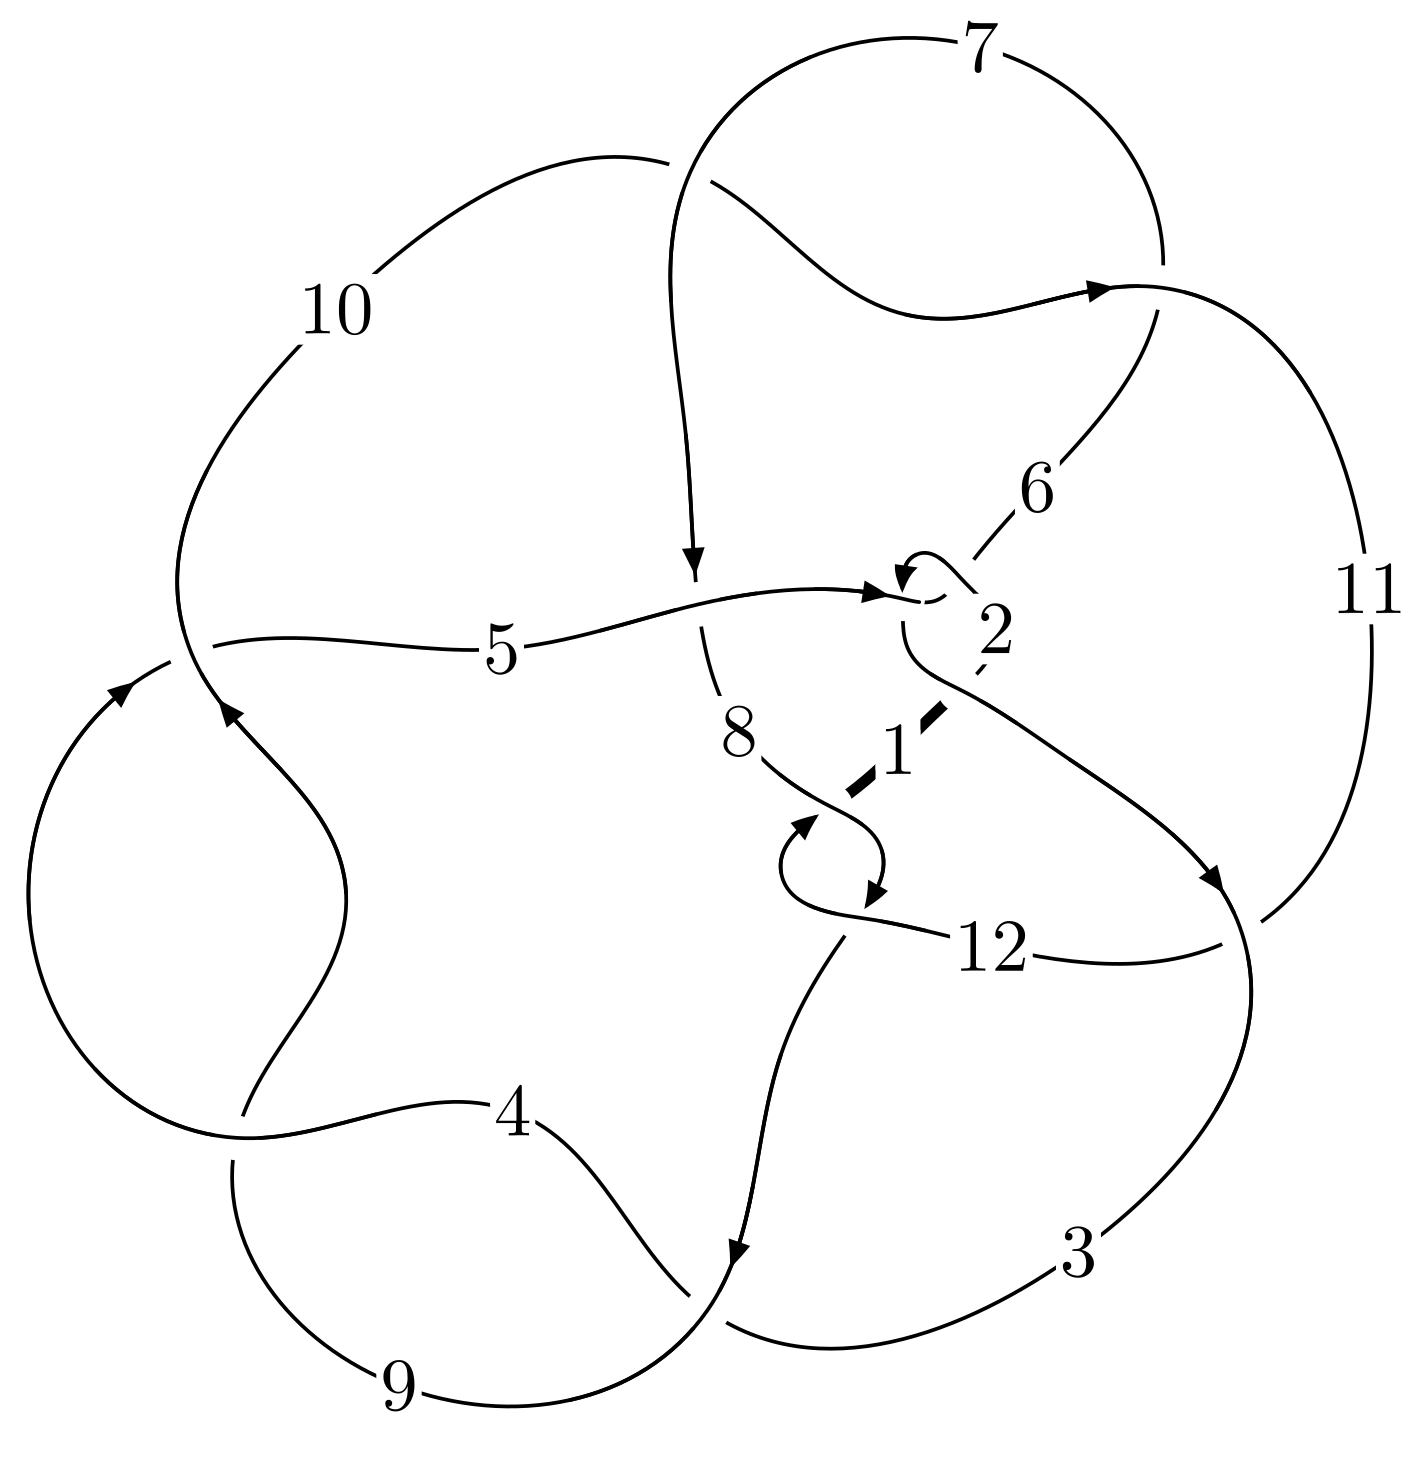
\includegraphics[width=112pt]{../../../GIT/diagram.site/Diagrams/png/2635_12n_0546.png}\\
\ \ \ A knot diagram\footnotemark}&
\allowdisplaybreaks
\textbf{Linearized knot diagam} \\
\cline{2-2}
 &
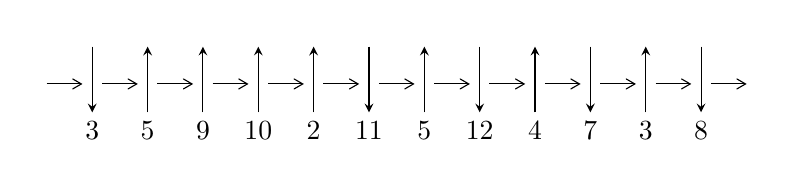
\begin{tikzpicture}[x=20pt, y=17pt]
	% nodes
	\node (C0) at (0, 0) {};
	\node (C1) at (1, 0) {};
	\node (C1U) at (1, +1) {};
	\node (C1D) at (1, -1) {3};

	\node (C2) at (2, 0) {};
	\node (C2U) at (2, +1) {};
	\node (C2D) at (2, -1) {5};

	\node (C3) at (3, 0) {};
	\node (C3U) at (3, +1) {};
	\node (C3D) at (3, -1) {9};

	\node (C4) at (4, 0) {};
	\node (C4U) at (4, +1) {};
	\node (C4D) at (4, -1) {10};

	\node (C5) at (5, 0) {};
	\node (C5U) at (5, +1) {};
	\node (C5D) at (5, -1) {2};

	\node (C6) at (6, 0) {};
	\node (C6U) at (6, +1) {};
	\node (C6D) at (6, -1) {11};

	\node (C7) at (7, 0) {};
	\node (C7U) at (7, +1) {};
	\node (C7D) at (7, -1) {5};

	\node (C8) at (8, 0) {};
	\node (C8U) at (8, +1) {};
	\node (C8D) at (8, -1) {12};

	\node (C9) at (9, 0) {};
	\node (C9U) at (9, +1) {};
	\node (C9D) at (9, -1) {4};

	\node (C10) at (10, 0) {};
	\node (C10U) at (10, +1) {};
	\node (C10D) at (10, -1) {7};

	\node (C11) at (11, 0) {};
	\node (C11U) at (11, +1) {};
	\node (C11D) at (11, -1) {3};

	\node (C12) at (12, 0) {};
	\node (C12U) at (12, +1) {};
	\node (C12D) at (12, -1) {8};
	\node (C13) at (13, 0) {};

	% arrows
	\draw[->,>={angle 60}]
	(C0) edge (C1) (C1) edge (C2) (C2) edge (C3) (C3) edge (C4) (C4) edge (C5) (C5) edge (C6) (C6) edge (C7) (C7) edge (C8) (C8) edge (C9) (C9) edge (C10) (C10) edge (C11) (C11) edge (C12) (C12) edge (C13) ;	\draw[->,>=stealth]
	(C1U) edge (C1D) (C2D) edge (C2U) (C3D) edge (C3U) (C4D) edge (C4U) (C5D) edge (C5U) (C6U) edge (C6D) (C7D) edge (C7U) (C8U) edge (C8D) (C9D) edge (C9U) (C10U) edge (C10D) (C11D) edge (C11U) (C12U) edge (C12D) ;
	\end{tikzpicture} \\
\hhline{~~} \\& 
\textbf{Solving Sequence} \\ \cline{2-2} 
 &
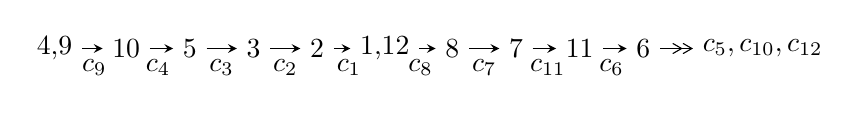
\begin{tikzpicture}[x=23pt, y=7pt]
	% node
	\node (A0) at (-1/8, 0) {4,9};
	\node (A1) at (1, 0) {10};
	\node (A2) at (2, 0) {5};
	\node (A3) at (3, 0) {3};
	\node (A4) at (4, 0) {2};
	\node (A5) at (81/16, 0) {1,12};
	\node (A6) at (49/8, 0) {8};
	\node (A7) at (57/8, 0) {7};
	\node (A8) at (65/8, 0) {11};
	\node (A9) at (73/8, 0) {6};
	\node (C1) at (1/2, -1) {$c_{9}$};
	\node (C2) at (3/2, -1) {$c_{4}$};
	\node (C3) at (5/2, -1) {$c_{3}$};
	\node (C4) at (7/2, -1) {$c_{2}$};
	\node (C5) at (9/2, -1) {$c_{1}$};
	\node (C6) at (45/8, -1) {$c_{8}$};
	\node (C7) at (53/8, -1) {$c_{7}$};
	\node (C8) at (61/8, -1) {$c_{11}$};
	\node (C9) at (69/8, -1) {$c_{6}$};
	\node (A10) at (11, 0) {$c_{5},c_{10},c_{12}$};

	% edge
	\draw[->,>=stealth]	
	(A0) edge (A1) (A1) edge (A2) (A2) edge (A3) (A3) edge (A4) (A4) edge (A5) (A5) edge (A6) (A6) edge (A7) (A7) edge (A8) (A8) edge (A9) ;
	\draw[->>,>={angle 60}]	
	(A9) edge (A10);
\end{tikzpicture} \\ 

\end{tabular} \\

\footnotetext{
The image of knot diagram is generated by the software ``\textbf{Draw programme}" developed by Andrew Bartholomew(\url{http://www.layer8.co.uk/maths/draw/index.htm\#Running-draw}), where we modified some parts for our purpose(\url{https://github.com/CATsTAILs/LinksPainter}).
}\phantom \\ \newline 
\centering \textbf{Ideals for irreducible components\footnotemark of $X_{\text{par}}$} 
 
\begin{align*}
I^u_{1}&=\langle 
u^{18}-2 u^{17}+\cdots+b-1,\;-3 u^{18}+5 u^{17}+\cdots+2 a+3,\;u^{19}-3 u^{18}+\cdots+u+2\rangle \\
I^u_{2}&=\langle 
3 u^9 a+3 u^9+\cdots- a+7,\;2 u^9 a+3 u^9+\cdots+3 a+9,\\
\phantom{I^u_{2}}&\phantom{= \langle  }u^{10}+u^9-5 u^8-4 u^7+8 u^6+3 u^5-5 u^4+2 u^3+3 u^2+u-1\rangle \\
I^u_{3}&=\langle 
- u^7+4 u^5-4 u^3+b,\;u^7-3 u^5+u^4+u^3-3 u^2+a+2 u+1,\;u^8-5 u^6+7 u^4-2 u^2+1\rangle \\
\\
\end{align*}
\raggedright * 3 irreducible components of $\dim_{\mathbb{C}}=0$, with total 47 representations.\\
\footnotetext{All coefficients of polynomials are rational numbers. But the coefficients are sometimes approximated in decimal forms when there is not enough margin.}
\newpage
\renewcommand{\arraystretch}{1}
\centering \section*{I. $I^u_{1}= \langle u^{18}-2 u^{17}+\cdots+b-1,\;-3 u^{18}+5 u^{17}+\cdots+2 a+3,\;u^{19}-3 u^{18}+\cdots+u+2 \rangle$}
\flushleft \textbf{(i) Arc colorings}\\
\begin{tabular}{m{7pt} m{180pt} m{7pt} m{180pt} }
\flushright $a_{4}=$&$\begin{pmatrix}0\\u\end{pmatrix}$ \\
\flushright $a_{9}=$&$\begin{pmatrix}1\\0\end{pmatrix}$ \\
\flushright $a_{10}=$&$\begin{pmatrix}1\\- u^2\end{pmatrix}$ \\
\flushright $a_{5}=$&$\begin{pmatrix}u\\- u^3+u\end{pmatrix}$ \\
\flushright $a_{3}=$&$\begin{pmatrix}- u\\u\end{pmatrix}$ \\
\flushright $a_{2}=$&$\begin{pmatrix}u^5-2 u^3- u\\- u^7+3 u^5-2 u^3+u\end{pmatrix}$ \\
\flushright $a_{1}=$&$\begin{pmatrix}- u^9+4 u^7-3 u^5-2 u^3- u\\u^9-5 u^7+7 u^5-2 u^3+u\end{pmatrix}$ \\
\flushright $a_{12}=$&$\begin{pmatrix}\frac{3}{2} u^{18}-\frac{5}{2} u^{17}+\cdots-\frac{5}{2} u-\frac{3}{2}\\- u^{18}+2 u^{17}+\cdots+2 u+1\end{pmatrix}$ \\
\flushright $a_{8}=$&$\begin{pmatrix}-\frac{1}{2} u^{18}+\frac{1}{2} u^{17}+\cdots-\frac{1}{2} u+\frac{1}{2}\\u^{18}- u^{17}+\cdots-2 u-1\end{pmatrix}$ \\
\flushright $a_{7}=$&$\begin{pmatrix}\frac{3}{2} u^{18}-\frac{5}{2} u^{17}+\cdots-\frac{5}{2} u-\frac{3}{2}\\-2 u^{18}+3 u^{17}+\cdots+3 u+3\end{pmatrix}$ \\
\flushright $a_{11}=$&$\begin{pmatrix}-\frac{1}{2} u^{18}+\frac{1}{2} u^{17}+\cdots-\frac{1}{2} u+\frac{1}{2}\\u^{18}- u^{17}+\cdots- u^2-1\end{pmatrix}$ \\
\flushright $a_{6}=$&$\begin{pmatrix}- u^9+4 u^7-3 u^5-2 u^3- u\\u^{11}-5 u^9+8 u^7-5 u^5+3 u^3- u\end{pmatrix}$\\&\end{tabular}
\flushleft \textbf{(ii) Obstruction class $= -1$}\\~\\
\flushleft \textbf{(iii) Cusp Shapes $= -4 u^{18}+4 u^{17}+38 u^{16}-28 u^{15}-150 u^{14}+56 u^{13}+322 u^{12}+22 u^{11}-400 u^{10}-208 u^9+252 u^8+260 u^7-22 u^6-128 u^5-46 u^4+12 u^3+16 u^2+12 u+10$}\\~\\
\newpage\renewcommand{\arraystretch}{1}
\flushleft \textbf{(iv) u-Polynomials at the component}\newline \\
\begin{tabular}{m{50pt}|m{274pt}}
Crossings & \hspace{64pt}u-Polynomials at each crossing \\
\hline $$\begin{aligned}c_{1}\end{aligned}$$&$\begin{aligned}
&u^{19}+15 u^{18}+\cdots+5217 u-64
\end{aligned}$\\
\hline $$\begin{aligned}c_{2},c_{5}\end{aligned}$$&$\begin{aligned}
&u^{19}+3 u^{18}+\cdots+55 u-8
\end{aligned}$\\
\hline $$\begin{aligned}c_{3},c_{4},c_{9}\end{aligned}$$&$\begin{aligned}
&u^{19}+3 u^{18}+\cdots+u-2
\end{aligned}$\\
\hline $$\begin{aligned}c_{6},c_{8},c_{10}\\c_{12}\end{aligned}$$&$\begin{aligned}
&u^{19}+2 u^{17}+\cdots-4 u^2-1
\end{aligned}$\\
\hline $$\begin{aligned}c_{7},c_{11}\end{aligned}$$&$\begin{aligned}
&u^{19}+4 u^{18}+\cdots-20 u+7
\end{aligned}$\\
\hline
\end{tabular}\\~\\
\newpage\renewcommand{\arraystretch}{1}
\flushleft \textbf{(v) Riley Polynomials at the component}\newline \\
\begin{tabular}{m{50pt}|m{274pt}}
Crossings & \hspace{64pt}Riley Polynomials at each crossing \\
\hline $$\begin{aligned}c_{1}\end{aligned}$$&$\begin{aligned}
&y^{19}-21 y^{18}+\cdots+25516865 y-4096
\end{aligned}$\\
\hline $$\begin{aligned}c_{2},c_{5}\end{aligned}$$&$\begin{aligned}
&y^{19}+15 y^{18}+\cdots+5217 y-64
\end{aligned}$\\
\hline $$\begin{aligned}c_{3},c_{4},c_{9}\end{aligned}$$&$\begin{aligned}
&y^{19}-21 y^{18}+\cdots-3 y-4
\end{aligned}$\\
\hline $$\begin{aligned}c_{6},c_{8},c_{10}\\c_{12}\end{aligned}$$&$\begin{aligned}
&y^{19}+4 y^{18}+\cdots-8 y-1
\end{aligned}$\\
\hline $$\begin{aligned}c_{7},c_{11}\end{aligned}$$&$\begin{aligned}
&y^{19}+20 y^{18}+\cdots-818 y-49
\end{aligned}$\\
\hline
\end{tabular}\\~\\
\newpage\flushleft \textbf{(vi) Complex Volumes and Cusp Shapes}
$$\begin{array}{c|c|c}  
\text{Solutions to }I^u_{1}& \I (\text{vol} + \sqrt{-1}CS) & \text{Cusp shape}\\
 \hline 
\begin{aligned}
u &= -0.580262 + 0.658546 I \\
a &= -1.37393 + 1.42710 I \\
b &= -0.88981 - 1.12332 I\end{aligned}
 & -6.36763 - 9.41239 I & \phantom{-}2.24569 + 7.34910 I \\ \hline\begin{aligned}
u &= -0.580262 - 0.658546 I \\
a &= -1.37393 - 1.42710 I \\
b &= -0.88981 + 1.12332 I\end{aligned}
 & -6.36763 + 9.41239 I & \phantom{-}2.24569 - 7.34910 I \\ \hline\begin{aligned}
u &= -0.430386 + 0.693344 I \\
a &= \phantom{-}0.0599143 - 0.0949401 I \\
b &= \phantom{-}0.92934 - 1.06686 I\end{aligned}
 & -6.81456 + 4.87246 I & \phantom{-}1.03546 - 1.73049 I \\ \hline\begin{aligned}
u &= -0.430386 - 0.693344 I \\
a &= \phantom{-}0.0599143 + 0.0949401 I \\
b &= \phantom{-}0.92934 + 1.06686 I\end{aligned}
 & -6.81456 - 4.87246 I & \phantom{-}1.03546 + 1.73049 I \\ \hline\begin{aligned}
u &= \phantom{-}0.736476 + 0.343968 I \\
a &= -0.27984 - 1.85203 I \\
b &= -0.603953 + 0.709870 I\end{aligned}
 & \phantom{-}1.05767 + 4.20616 I & \phantom{-}4.94312 - 8.38858 I \\ \hline\begin{aligned}
u &= \phantom{-}0.736476 - 0.343968 I \\
a &= -0.27984 + 1.85203 I \\
b &= -0.603953 - 0.709870 I\end{aligned}
 & \phantom{-}1.05767 - 4.20616 I & \phantom{-}4.94312 + 8.38858 I \\ \hline\begin{aligned}
u &= -0.609189 + 0.322877 I \\
a &= \phantom{-}0.730128 - 0.841386 I \\
b &= -0.206405 + 0.511932 I\end{aligned}
 & \phantom{-}1.17956 - 0.90815 I & \phantom{-}4.85874 + 1.33440 I \\ \hline\begin{aligned}
u &= -0.609189 - 0.322877 I \\
a &= \phantom{-}0.730128 + 0.841386 I \\
b &= -0.206405 - 0.511932 I\end{aligned}
 & \phantom{-}1.17956 + 0.90815 I & \phantom{-}4.85874 - 1.33440 I \\ \hline\begin{aligned}
u &= -1.39358\phantom{ +0.000000I} \\
a &= \phantom{-}0.388481\phantom{ +0.000000I} \\
b &= -0.879243\phantom{ +0.000000I}\end{aligned}
 & \phantom{-}3.32984\phantom{ +0.000000I} & \phantom{-}1.51140\phantom{ +0.000000I} \\ \hline\begin{aligned}
u &= \phantom{-}1.45691 + 0.21847 I \\
a &= \phantom{-}0.750156 + 0.704154 I \\
b &= -0.975115 - 0.981574 I\end{aligned}
 & -0.73866 - 1.59783 I & \phantom{-}4.12138 + 1.54661 I\\
 \hline 
 \end{array}$$\newpage$$\begin{array}{c|c|c}  
\text{Solutions to }I^u_{1}& \I (\text{vol} + \sqrt{-1}CS) & \text{Cusp shape}\\
 \hline 
\begin{aligned}
u &= \phantom{-}1.45691 - 0.21847 I \\
a &= \phantom{-}0.750156 - 0.704154 I \\
b &= -0.975115 + 0.981574 I\end{aligned}
 & -0.73866 + 1.59783 I & \phantom{-}4.12138 - 1.54661 I \\ \hline\begin{aligned}
u &= \phantom{-}0.094599 + 0.501708 I \\
a &= \phantom{-}0.412228 - 0.106777 I \\
b &= \phantom{-}0.620442 + 0.453397 I\end{aligned}
 & -0.91663 - 1.23074 I & -2.16741 + 3.03279 I \\ \hline\begin{aligned}
u &= \phantom{-}0.094599 - 0.501708 I \\
a &= \phantom{-}0.412228 + 0.106777 I \\
b &= \phantom{-}0.620442 - 0.453397 I\end{aligned}
 & -0.91663 + 1.23074 I & -2.16741 - 3.03279 I \\ \hline\begin{aligned}
u &= \phantom{-}1.55341 + 0.21071 I \\
a &= \phantom{-}0.57402 + 2.23414 I \\
b &= \phantom{-}0.84741 - 1.16742 I\end{aligned}
 & \phantom{-}0.68963 + 12.60340 I & \phantom{-}5.72673 - 6.88576 I \\ \hline\begin{aligned}
u &= \phantom{-}1.55341 - 0.21071 I \\
a &= \phantom{-}0.57402 - 2.23414 I \\
b &= \phantom{-}0.84741 + 1.16742 I\end{aligned}
 & \phantom{-}0.68963 - 12.60340 I & \phantom{-}5.72673 + 6.88576 I \\ \hline\begin{aligned}
u &= \phantom{-}1.57600 + 0.10063 I \\
a &= -0.61810 - 1.45739 I \\
b &= \phantom{-}0.193132 + 0.647212 I\end{aligned}
 & \phantom{-}8.62226 + 2.51189 I & \phantom{-}5.75786 + 1.20779 I \\ \hline\begin{aligned}
u &= \phantom{-}1.57600 - 0.10063 I \\
a &= -0.61810 + 1.45739 I \\
b &= \phantom{-}0.193132 - 0.647212 I\end{aligned}
 & \phantom{-}8.62226 - 2.51189 I & \phantom{-}5.75786 - 1.20779 I \\ \hline\begin{aligned}
u &= -1.60077 + 0.07995 I \\
a &= -0.19881 - 2.15189 I \\
b &= \phantom{-}0.524578 + 0.835989 I\end{aligned}
 & \phantom{-}9.02564 - 5.69404 I & \phantom{-}7.72276 + 7.13841 I \\ \hline\begin{aligned}
u &= -1.60077 - 0.07995 I \\
a &= -0.19881 + 2.15189 I \\
b &= \phantom{-}0.524578 - 0.835989 I\end{aligned}
 & \phantom{-}9.02564 + 5.69404 I & \phantom{-}7.72276 - 7.13841 I\\
 \hline 
 \end{array}$$\newpage\newpage\renewcommand{\arraystretch}{1}
\centering \section*{II. $I^u_{2}= \langle 3 u^9 a+3 u^9+\cdots- a+7,\;2 u^9 a+3 u^9+\cdots+3 a+9,\;u^{10}+u^9+\cdots+u-1 \rangle$}
\flushleft \textbf{(i) Arc colorings}\\
\begin{tabular}{m{7pt} m{180pt} m{7pt} m{180pt} }
\flushright $a_{4}=$&$\begin{pmatrix}0\\u\end{pmatrix}$ \\
\flushright $a_{9}=$&$\begin{pmatrix}1\\0\end{pmatrix}$ \\
\flushright $a_{10}=$&$\begin{pmatrix}1\\- u^2\end{pmatrix}$ \\
\flushright $a_{5}=$&$\begin{pmatrix}u\\- u^3+u\end{pmatrix}$ \\
\flushright $a_{3}=$&$\begin{pmatrix}- u\\u\end{pmatrix}$ \\
\flushright $a_{2}=$&$\begin{pmatrix}u^5-2 u^3- u\\- u^7+3 u^5-2 u^3+u\end{pmatrix}$ \\
\flushright $a_{1}=$&$\begin{pmatrix}- u^9+4 u^7-3 u^5-2 u^3- u\\u^9-5 u^7+7 u^5-2 u^3+u\end{pmatrix}$ \\
\flushright $a_{12}=$&$\begin{pmatrix}a\\-\frac{3}{8} u^9 a-\frac{3}{8} u^9+\cdots+\frac{1}{8} a-\frac{7}{8}\end{pmatrix}$ \\
\flushright $a_{8}=$&$\begin{pmatrix}-\frac{3}{8} u^9 a-\frac{3}{8} u^9+\cdots-\frac{7}{8} a-\frac{23}{8}\\-\frac{3}{8} u^9 a-\frac{3}{8} u^9+\cdots+\frac{1}{8} a+\frac{9}{8}\end{pmatrix}$ \\
\flushright $a_{7}=$&$\begin{pmatrix}-2 u^9-2 u^8+8 u^7+8 u^6-8 u^5-8 u^4+2 u^3+u^2- a-6 u-3\\-\frac{3}{8} u^9 a+\frac{13}{8} u^9+\cdots+\frac{1}{8} a-\frac{7}{8}\end{pmatrix}$ \\
\flushright $a_{11}=$&$\begin{pmatrix}\frac{3}{8} u^9 a+\frac{3}{8} u^9+\cdots+\frac{7}{8} a-\frac{1}{8}\\-\frac{3}{4} u^9 a-\frac{3}{4} u^9+\cdots+\frac{1}{4} a-\frac{3}{4}\end{pmatrix}$ \\
\flushright $a_{6}=$&$\begin{pmatrix}- u^9+4 u^7-3 u^5-2 u^3- u\\u^9- u^8-4 u^7+5 u^6+3 u^5-7 u^4+2 u^3+2 u^2+u-1\end{pmatrix}$\\&\end{tabular}
\flushleft \textbf{(ii) Obstruction class $= -1$}\\~\\
\flushleft \textbf{(iii) Cusp Shapes $= 4 u^8-20 u^6+28 u^4-4 u^3-8 u^2+8 u+10$}\\~\\
\newpage\renewcommand{\arraystretch}{1}
\flushleft \textbf{(iv) u-Polynomials at the component}\newline \\
\begin{tabular}{m{50pt}|m{274pt}}
Crossings & \hspace{64pt}u-Polynomials at each crossing \\
\hline $$\begin{aligned}c_{1}\end{aligned}$$&$\begin{aligned}
&(u^{10}+13 u^9+\cdots-7 u+1)^{2}
\end{aligned}$\\
\hline $$\begin{aligned}c_{2},c_{5}\end{aligned}$$&$\begin{aligned}
&(u^{10}+u^9+7 u^8+6 u^7+16 u^6+11 u^5+13 u^4+6 u^3+3 u^2+u-1)^2
\end{aligned}$\\
\hline $$\begin{aligned}c_{3},c_{4},c_{9}\end{aligned}$$&$\begin{aligned}
&(u^{10}- u^9-5 u^8+4 u^7+8 u^6-3 u^5-5 u^4-2 u^3+3 u^2- u-1)^2
\end{aligned}$\\
\hline $$\begin{aligned}c_{6},c_{8},c_{10}\\c_{12}\end{aligned}$$&$\begin{aligned}
&u^{20}+u^{19}+\cdots- u+2
\end{aligned}$\\
\hline $$\begin{aligned}c_{7},c_{11}\end{aligned}$$&$\begin{aligned}
&u^{20}+u^{19}+\cdots+637 u+1708
\end{aligned}$\\
\hline
\end{tabular}\\~\\
\newpage\renewcommand{\arraystretch}{1}
\flushleft \textbf{(v) Riley Polynomials at the component}\newline \\
\begin{tabular}{m{50pt}|m{274pt}}
Crossings & \hspace{64pt}Riley Polynomials at each crossing \\
\hline $$\begin{aligned}c_{1}\end{aligned}$$&$\begin{aligned}
&(y^{10}-31 y^9+\cdots-107 y+1)^{2}
\end{aligned}$\\
\hline $$\begin{aligned}c_{2},c_{5}\end{aligned}$$&$\begin{aligned}
&(y^{10}+13 y^9+\cdots-7 y+1)^{2}
\end{aligned}$\\
\hline $$\begin{aligned}c_{3},c_{4},c_{9}\end{aligned}$$&$\begin{aligned}
&(y^{10}-11 y^9+\cdots-7 y+1)^{2}
\end{aligned}$\\
\hline $$\begin{aligned}c_{6},c_{8},c_{10}\\c_{12}\end{aligned}$$&$\begin{aligned}
&y^{20}+7 y^{19}+\cdots+35 y+4
\end{aligned}$\\
\hline $$\begin{aligned}c_{7},c_{11}\end{aligned}$$&$\begin{aligned}
&y^{20}- y^{19}+\cdots-641473 y+2917264
\end{aligned}$\\
\hline
\end{tabular}\\~\\
\newpage\flushleft \textbf{(vi) Complex Volumes and Cusp Shapes}
$$\begin{array}{c|c|c}  
\text{Solutions to }I^u_{2}& \I (\text{vol} + \sqrt{-1}CS) & \text{Cusp shape}\\
 \hline 
\begin{aligned}
u &= \phantom{-}0.510102 + 0.680941 I \\
a &= \phantom{-}1.03901 + 0.99672 I \\
b &= \phantom{-}1.030620 - 0.877048 I\end{aligned}
 & -7.43042 + 2.28632 I & \phantom{-}0.39779 - 2.91176 I \\ \hline\begin{aligned}
u &= \phantom{-}0.510102 + 0.680941 I \\
a &= \phantom{-}0.139978 - 0.495824 I \\
b &= -1.064860 - 0.795059 I\end{aligned}
 & -7.43042 + 2.28632 I & \phantom{-}0.39779 - 2.91176 I \\ \hline\begin{aligned}
u &= \phantom{-}0.510102 - 0.680941 I \\
a &= \phantom{-}1.03901 - 0.99672 I \\
b &= \phantom{-}1.030620 + 0.877048 I\end{aligned}
 & -7.43042 - 2.28632 I & \phantom{-}0.39779 + 2.91176 I \\ \hline\begin{aligned}
u &= \phantom{-}0.510102 - 0.680941 I \\
a &= \phantom{-}0.139978 + 0.495824 I \\
b &= -1.064860 + 0.795059 I\end{aligned}
 & -7.43042 - 2.28632 I & \phantom{-}0.39779 + 2.91176 I \\ \hline\begin{aligned}
u &= -0.449833 + 0.459351 I \\
a &= -0.646997 - 0.974683 I \\
b &= -0.210455 - 0.300293 I\end{aligned}
 & \phantom{-}1.43061 - 1.60532 I & \phantom{-}0.94346 + 5.03395 I \\ \hline\begin{aligned}
u &= -0.449833 + 0.459351 I \\
a &= \phantom{-}1.22866 - 0.93250 I \\
b &= \phantom{-}0.057050 + 1.133970 I\end{aligned}
 & \phantom{-}1.43061 - 1.60532 I & \phantom{-}0.94346 + 5.03395 I \\ \hline\begin{aligned}
u &= -0.449833 - 0.459351 I \\
a &= -0.646997 + 0.974683 I \\
b &= -0.210455 + 0.300293 I\end{aligned}
 & \phantom{-}1.43061 + 1.60532 I & \phantom{-}0.94346 - 5.03395 I \\ \hline\begin{aligned}
u &= -0.449833 - 0.459351 I \\
a &= \phantom{-}1.22866 + 0.93250 I \\
b &= \phantom{-}0.057050 - 1.133970 I\end{aligned}
 & \phantom{-}1.43061 + 1.60532 I & \phantom{-}0.94346 - 5.03395 I \\ \hline\begin{aligned}
u &= \phantom{-}1.50079 + 0.11328 I \\
a &= \phantom{-}0.415489 - 0.034479 I \\
b &= \phantom{-}0.528203 - 0.415736 I\end{aligned}
 & \phantom{-}7.87146 + 3.55946 I & \phantom{-}5.64226 - 4.06361 I \\ \hline\begin{aligned}
u &= \phantom{-}1.50079 + 0.11328 I \\
a &= -0.70682 - 2.20481 I \\
b &= -0.107369 + 1.258670 I\end{aligned}
 & \phantom{-}7.87146 + 3.55946 I & \phantom{-}5.64226 - 4.06361 I\\
 \hline 
 \end{array}$$\newpage$$\begin{array}{c|c|c}  
\text{Solutions to }I^u_{2}& \I (\text{vol} + \sqrt{-1}CS) & \text{Cusp shape}\\
 \hline 
\begin{aligned}
u &= \phantom{-}1.50079 - 0.11328 I \\
a &= \phantom{-}0.415489 + 0.034479 I \\
b &= \phantom{-}0.528203 + 0.415736 I\end{aligned}
 & \phantom{-}7.87146 - 3.55946 I & \phantom{-}5.64226 + 4.06361 I \\ \hline\begin{aligned}
u &= \phantom{-}1.50079 - 0.11328 I \\
a &= -0.70682 + 2.20481 I \\
b &= -0.107369 - 1.258670 I\end{aligned}
 & \phantom{-}7.87146 - 3.55946 I & \phantom{-}5.64226 + 4.06361 I \\ \hline\begin{aligned}
u &= -1.50960\phantom{ +0.000000I} \\
a &= \phantom{-}0.93389 + 2.29683 I \\
b &= \phantom{-}0.317795 - 1.141480 I\end{aligned}
 & \phantom{-}10.4232\phantom{ +0.000000I} & \phantom{-}10.0490\phantom{ +0.000000I} \\ \hline\begin{aligned}
u &= -1.50960\phantom{ +0.000000I} \\
a &= \phantom{-}0.93389 - 2.29683 I \\
b &= \phantom{-}0.317795 + 1.141480 I\end{aligned}
 & \phantom{-}10.4232\phantom{ +0.000000I} & \phantom{-}10.0490\phantom{ +0.000000I} \\ \hline\begin{aligned}
u &= -1.51481 + 0.22020 I \\
a &= -0.956858 + 0.125386 I \\
b &= \phantom{-}1.093790 - 0.701969 I\end{aligned}
 & -0.80829 - 5.55652 I & \phantom{-}3.79190 + 2.88175 I \\ \hline\begin{aligned}
u &= -1.51481 + 0.22020 I \\
a &= -0.21158 + 1.73958 I \\
b &= -0.985922 - 0.960677 I\end{aligned}
 & -0.80829 - 5.55652 I & \phantom{-}3.79190 + 2.88175 I \\ \hline\begin{aligned}
u &= -1.51481 - 0.22020 I \\
a &= -0.956858 - 0.125386 I \\
b &= \phantom{-}1.093790 + 0.701969 I\end{aligned}
 & -0.80829 + 5.55652 I & \phantom{-}3.79190 - 2.88175 I \\ \hline\begin{aligned}
u &= -1.51481 - 0.22020 I \\
a &= -0.21158 - 1.73958 I \\
b &= -0.985922 + 0.960677 I\end{aligned}
 & -0.80829 + 5.55652 I & \phantom{-}3.79190 - 2.88175 I \\ \hline\begin{aligned}
u &= \phantom{-}0.417104\phantom{ +0.000000I} \\
a &= -2.73478 + 2.69676 I \\
b &= -0.158842 - 1.037160 I\end{aligned}
 & \phantom{-}3.89939\phantom{ +0.000000I} & \phantom{-}12.4010\phantom{ +0.000000I} \\ \hline\begin{aligned}
u &= \phantom{-}0.417104\phantom{ +0.000000I} \\
a &= -2.73478 - 2.69676 I \\
b &= -0.158842 + 1.037160 I\end{aligned}
 & \phantom{-}3.89939\phantom{ +0.000000I} & \phantom{-}12.4010\phantom{ +0.000000I}\\
 \hline 
 \end{array}$$\newpage\newpage\renewcommand{\arraystretch}{1}
\centering \section*{III. $I^u_{3}= \langle - u^7+4 u^5-4 u^3+b,\;u^7-3 u^5+u^4+u^3-3 u^2+a+2 u+1,\;u^8-5 u^6+7 u^4-2 u^2+1 \rangle$}
\flushleft \textbf{(i) Arc colorings}\\
\begin{tabular}{m{7pt} m{180pt} m{7pt} m{180pt} }
\flushright $a_{4}=$&$\begin{pmatrix}0\\u\end{pmatrix}$ \\
\flushright $a_{9}=$&$\begin{pmatrix}1\\0\end{pmatrix}$ \\
\flushright $a_{10}=$&$\begin{pmatrix}1\\- u^2\end{pmatrix}$ \\
\flushright $a_{5}=$&$\begin{pmatrix}u\\- u^3+u\end{pmatrix}$ \\
\flushright $a_{3}=$&$\begin{pmatrix}- u\\u\end{pmatrix}$ \\
\flushright $a_{2}=$&$\begin{pmatrix}u^5-2 u^3- u\\- u^7+3 u^5-2 u^3+u\end{pmatrix}$ \\
\flushright $a_{1}=$&$\begin{pmatrix}- u^7+4 u^5-4 u^3\\0\end{pmatrix}$ \\
\flushright $a_{12}=$&$\begin{pmatrix}- u^7+3 u^5- u^4- u^3+3 u^2-2 u-1\\u^7-4 u^5+4 u^3\end{pmatrix}$ \\
\flushright $a_{8}=$&$\begin{pmatrix}u^6-4 u^4- u^3+4 u^2+2 u-1\\1\end{pmatrix}$ \\
\flushright $a_{7}=$&$\begin{pmatrix}u^7-3 u^5- u^4+u^3+3 u^2+2 u-1\\- u^7+u^6+2 u^5-3 u^4+u^2+u\end{pmatrix}$ \\
\flushright $a_{11}=$&$\begin{pmatrix}u^6-4 u^4+u^3+4 u^2-2 u-1\\- u^6- u^5+3 u^4+2 u^3- u^2\end{pmatrix}$ \\
\flushright $a_{6}=$&$\begin{pmatrix}u^7-4 u^5+4 u^3\\- u^7+3 u^5-2 u^3+u\end{pmatrix}$\\&\end{tabular}
\flushleft \textbf{(ii) Obstruction class $= 1$}\\~\\
\flushleft \textbf{(iii) Cusp Shapes $= -4 u^6+16 u^4-16 u^2+12$}\\~\\
\newpage\renewcommand{\arraystretch}{1}
\flushleft \textbf{(iv) u-Polynomials at the component}\newline \\
\begin{tabular}{m{50pt}|m{274pt}}
Crossings & \hspace{64pt}u-Polynomials at each crossing \\
\hline $$\begin{aligned}c_{1}\end{aligned}$$&$\begin{aligned}
&(u^4- u^3+3 u^2-2 u+1)^2
\end{aligned}$\\
\hline $$\begin{aligned}c_{2}\end{aligned}$$&$\begin{aligned}
&(u^4- u^3+u^2+1)^2
\end{aligned}$\\
\hline $$\begin{aligned}c_{3},c_{4},c_{9}\end{aligned}$$&$\begin{aligned}
&u^8-5 u^6+7 u^4-2 u^2+1
\end{aligned}$\\
\hline $$\begin{aligned}c_{5}\end{aligned}$$&$\begin{aligned}
&(u^4+u^3+u^2+1)^2
\end{aligned}$\\
\hline $$\begin{aligned}c_{6},c_{8},c_{10}\\c_{12}\end{aligned}$$&$\begin{aligned}
&(u^2+1)^4
\end{aligned}$\\
\hline $$\begin{aligned}c_{7}\end{aligned}$$&$\begin{aligned}
&u^8-6 u^7+20 u^6-52 u^5+97 u^4-112 u^3+87 u^2-62 u+29
\end{aligned}$\\
\hline $$\begin{aligned}c_{11}\end{aligned}$$&$\begin{aligned}
&u^8+6 u^7+20 u^6+52 u^5+97 u^4+112 u^3+87 u^2+62 u+29
\end{aligned}$\\
\hline
\end{tabular}\\~\\
\newpage\renewcommand{\arraystretch}{1}
\flushleft \textbf{(v) Riley Polynomials at the component}\newline \\
\begin{tabular}{m{50pt}|m{274pt}}
Crossings & \hspace{64pt}Riley Polynomials at each crossing \\
\hline $$\begin{aligned}c_{1}\end{aligned}$$&$\begin{aligned}
&(y^4+5 y^3+7 y^2+2 y+1)^2
\end{aligned}$\\
\hline $$\begin{aligned}c_{2},c_{5}\end{aligned}$$&$\begin{aligned}
&(y^4+y^3+3 y^2+2 y+1)^2
\end{aligned}$\\
\hline $$\begin{aligned}c_{3},c_{4},c_{9}\end{aligned}$$&$\begin{aligned}
&(y^4-5 y^3+7 y^2-2 y+1)^2
\end{aligned}$\\
\hline $$\begin{aligned}c_{6},c_{8},c_{10}\\c_{12}\end{aligned}$$&$\begin{aligned}
&(y+1)^8
\end{aligned}$\\
\hline $$\begin{aligned}c_{7},c_{11}\end{aligned}$$&$\begin{aligned}
&y^8+4 y^7-30 y^6+6 y^5+555 y^4-954 y^3-693 y^2+1202 y+841
\end{aligned}$\\
\hline
\end{tabular}\\~\\
\newpage\flushleft \textbf{(vi) Complex Volumes and Cusp Shapes}
$$\begin{array}{c|c|c}  
\text{Solutions to }I^u_{3}& \I (\text{vol} + \sqrt{-1}CS) & \text{Cusp shape}\\
 \hline 
\begin{aligned}
u &= \phantom{-}0.506844 + 0.395123 I \\
a &= -1.77461 + 0.07756 I \\
b &= \phantom{-0.000000 -}1.000000 I\end{aligned}
 & \phantom{-}3.07886 + 1.41510 I & \phantom{-}8.17326 - 4.90874 I \\ \hline\begin{aligned}
u &= \phantom{-}0.506844 - 0.395123 I \\
a &= -1.77461 - 0.07756 I \\
b &= \phantom{-0.000000 } -1.000000 I\end{aligned}
 & \phantom{-}3.07886 - 1.41510 I & \phantom{-}8.17326 + 4.90874 I \\ \hline\begin{aligned}
u &= -0.506844 + 0.395123 I \\
a &= \phantom{-}0.67976 - 2.16419 I \\
b &= \phantom{-0.000000 -}1.000000 I\end{aligned}
 & \phantom{-}3.07886 - 1.41510 I & \phantom{-}8.17326 + 4.90874 I \\ \hline\begin{aligned}
u &= -0.506844 - 0.395123 I \\
a &= \phantom{-}0.67976 + 2.16419 I \\
b &= \phantom{-0.000000 } -1.000000 I\end{aligned}
 & \phantom{-}3.07886 + 1.41510 I & \phantom{-}8.17326 - 4.90874 I \\ \hline\begin{aligned}
u &= \phantom{-}1.55249 + 0.10488 I \\
a &= -0.09378 - 2.54234 I \\
b &= \phantom{-0.000000 -}1.000000 I\end{aligned}
 & \phantom{-}10.08060 + 3.16396 I & \phantom{-}11.82674 - 2.56480 I \\ \hline\begin{aligned}
u &= \phantom{-}1.55249 - 0.10488 I \\
a &= -0.09378 + 2.54234 I \\
b &= \phantom{-0.000000 } -1.000000 I\end{aligned}
 & \phantom{-}10.08060 - 3.16396 I & \phantom{-}11.82674 + 2.56480 I \\ \hline\begin{aligned}
u &= -1.55249 + 0.10488 I \\
a &= \phantom{-}1.18862 - 1.37103 I \\
b &= \phantom{-0.000000 -}1.000000 I\end{aligned}
 & \phantom{-}10.08060 - 3.16396 I & \phantom{-}11.82674 + 2.56480 I \\ \hline\begin{aligned}
u &= -1.55249 - 0.10488 I \\
a &= \phantom{-}1.18862 + 1.37103 I \\
b &= \phantom{-0.000000 } -1.000000 I\end{aligned}
 & \phantom{-}10.08060 + 3.16396 I & \phantom{-}11.82674 - 2.56480 I\\
 \hline 
 \end{array}$$\newpage
\newpage\renewcommand{\arraystretch}{1}
\centering \section*{ IV. u-Polynomials}
\begin{tabular}{m{50pt}|m{274pt}}
Crossings & \hspace{64pt}u-Polynomials at each crossing \\
\hline $$\begin{aligned}c_{1}\end{aligned}$$&$\begin{aligned}
&((u^4- u^3+3 u^2-2 u+1)^2)(u^{10}+13 u^9+\cdots-7 u+1)^{2}\\
&\cdot(u^{19}+15 u^{18}+\cdots+5217 u-64)
\end{aligned}$\\
\hline $$\begin{aligned}c_{2}\end{aligned}$$&$\begin{aligned}
&(u^4- u^3+u^2+1)^2\\
&\cdot(u^{10}+u^9+7 u^8+6 u^7+16 u^6+11 u^5+13 u^4+6 u^3+3 u^2+u-1)^2\\
&\cdot(u^{19}+3 u^{18}+\cdots+55 u-8)
\end{aligned}$\\
\hline $$\begin{aligned}c_{3},c_{4},c_{9}\end{aligned}$$&$\begin{aligned}
&(u^8-5 u^6+7 u^4-2 u^2+1)\\
&\cdot(u^{10}- u^9-5 u^8+4 u^7+8 u^6-3 u^5-5 u^4-2 u^3+3 u^2- u-1)^2\\
&\cdot(u^{19}+3 u^{18}+\cdots+u-2)
\end{aligned}$\\
\hline $$\begin{aligned}c_{5}\end{aligned}$$&$\begin{aligned}
&(u^4+u^3+u^2+1)^2\\
&\cdot(u^{10}+u^9+7 u^8+6 u^7+16 u^6+11 u^5+13 u^4+6 u^3+3 u^2+u-1)^2\\
&\cdot(u^{19}+3 u^{18}+\cdots+55 u-8)
\end{aligned}$\\
\hline $$\begin{aligned}c_{6},c_{8},c_{10}\\c_{12}\end{aligned}$$&$\begin{aligned}
&((u^2+1)^4)(u^{19}+2 u^{17}+\cdots-4 u^2-1)(u^{20}+u^{19}+\cdots- u+2)
\end{aligned}$\\
\hline $$\begin{aligned}c_{7}\end{aligned}$$&$\begin{aligned}
&(u^8-6 u^7+20 u^6-52 u^5+97 u^4-112 u^3+87 u^2-62 u+29)\\
&\cdot(u^{19}+4 u^{18}+\cdots-20 u+7)(u^{20}+u^{19}+\cdots+637 u+1708)
\end{aligned}$\\
\hline $$\begin{aligned}c_{11}\end{aligned}$$&$\begin{aligned}
&(u^8+6 u^7+20 u^6+52 u^5+97 u^4+112 u^3+87 u^2+62 u+29)\\
&\cdot(u^{19}+4 u^{18}+\cdots-20 u+7)(u^{20}+u^{19}+\cdots+637 u+1708)
\end{aligned}$\\
\hline
\end{tabular}\newpage\renewcommand{\arraystretch}{1}
\centering \section*{ V. Riley Polynomials}
\begin{tabular}{m{50pt}|m{274pt}}
Crossings & \hspace{64pt}Riley Polynomials at each crossing \\
\hline $$\begin{aligned}c_{1}\end{aligned}$$&$\begin{aligned}
&((y^4+5 y^3+7 y^2+2 y+1)^2)(y^{10}-31 y^9+\cdots-107 y+1)^{2}\\
&\cdot(y^{19}-21 y^{18}+\cdots+25516865 y-4096)
\end{aligned}$\\
\hline $$\begin{aligned}c_{2},c_{5}\end{aligned}$$&$\begin{aligned}
&((y^4+y^3+3 y^2+2 y+1)^2)(y^{10}+13 y^9+\cdots-7 y+1)^{2}\\
&\cdot(y^{19}+15 y^{18}+\cdots+5217 y-64)
\end{aligned}$\\
\hline $$\begin{aligned}c_{3},c_{4},c_{9}\end{aligned}$$&$\begin{aligned}
&((y^4-5 y^3+7 y^2-2 y+1)^2)(y^{10}-11 y^9+\cdots-7 y+1)^{2}\\
&\cdot(y^{19}-21 y^{18}+\cdots-3 y-4)
\end{aligned}$\\
\hline $$\begin{aligned}c_{6},c_{8},c_{10}\\c_{12}\end{aligned}$$&$\begin{aligned}
&((y+1)^8)(y^{19}+4 y^{18}+\cdots-8 y-1)(y^{20}+7 y^{19}+\cdots+35 y+4)
\end{aligned}$\\
\hline $$\begin{aligned}c_{7},c_{11}\end{aligned}$$&$\begin{aligned}
&(y^8+4 y^7-30 y^6+6 y^5+555 y^4-954 y^3-693 y^2+1202 y+841)\\
&\cdot(y^{19}+20 y^{18}+\cdots-818 y-49)\\
&\cdot(y^{20}- y^{19}+\cdots-641473 y+2917264)
\end{aligned}$\\
\hline
\end{tabular}
\vskip 2pc
\end{document}